\documentclass[12pt]{article}

% Load packages
\usepackage[top=1in, bottom=1in, left=1in, right=1in]{geometry}
\usepackage{graphics}
\usepackage{graphicx}
\usepackage{epsfig}
\usepackage{epsf}
\usepackage{epstopdf}
\usepackage{mathrsfs}
\usepackage{amsmath}
\usepackage{amssymb}
\usepackage{textcomp}
\usepackage[scaled=.90]{helvet} % Helvetica (currently not used)
\usepackage[]{lineno} % For line numbers
\usepackage{natbib}

% Define new commands and definitions
\def\ds{\displaystyle}
\def\d{\partial}
\newcommand{\rr}{\mathbb{R}}
\newcommand{\zz}{\mathbb{Z}}
\newcommand{\nn}{\mathbb{N}}
\newcommand{\ee}{\mathscr{E}}
\newcommand{\mb}{\mathbf}
\newcommand{\ol}{\overline}

% Text formatting
\linespread 2	
\linenumbers

\title{Escape direction does not matter for some fish prey}
\author{Matthew J. McHenry, Alberto Soto}
%\date{}                                           % Activate to display a given date or no date

\begin{document}
\DeclareGraphicsExtensions{.eps,.pdf,.png,.gif,.jpg,.ps}

\maketitle

\pagebreak


% ABSTRACT
% --------------------------------------------------------------------------------
\begin{abstract}

Abstract text...

\end{abstract}

\pagebreak


% --------------------------------------------------------------------------------
\section{Introduction}

%TODO: Add citations to the intro

Biologists have long-appreciated the importance of predation in the ecology and evolution of prey species. This subject is extensive enough to fill the pages of books on the fascinating diversity of strategies that prey use to avoid encounters with predators (CITE) or to defend themselves when discovered (CITE). In contrast, our understanding for how prey evade capture by locomotion is relatively rudimentary. Although numerous studies have speculated on the importance of locomotor performance to survival, relatively few have examined what aspect of locomotion are most meaningful in these interactions. Studies that have explored this subject emphasize the common-sense notion that the direction of an escape matters to a prey's survival (CITE). It follows that the ability to move in a favorable direction depends on how well a prey can sense and respond to a predator with an evasive maneuver. The present paper considers these sensory-motor dynamics in prey fish in the context of a prey's evasion strategy. This is achieved by offering a new interpretation of a game-theory model for piscivorous interactions \citep{Weihs:1984tb} and relating the predictions of this model to experimental measurements of larval zebrafish (\textit{Danio rerio}) \citep{Stewart:2014cm}.

Game-theory models offer a basis for examining the strategic implications of locomotor behavior. One of the major aims of these models is to determine the optimal strategy of prey. The strategy is generally apparent in the direction of locomotion adopted when the predator is detected. There is recent interest in revisiting these modes with experimental studies that include both predators and prey. This includes work on terrestrial vertebrates (CITE), birds (CITE), bats (CITE), flying insects (CITE), zooplankton (CITE), and fishes (CITE). These efforts offer the potential to reveal how sensory and motor systems govern the outcome of predator-prey interactions. 

Piscivorous interactions offer some advantages for examining the sensory-motor basis of predator evasion. Many predatory fishes will attempt to feed on prey in a laboratory with motion that is largely two-dimensional and therefore relatively easy to measure. Zebrafish do this (CITE) and it is a species that offers a growing wealth of understanding in physiology (CITE) and neuroscience (CITE) that may be leveraged for mechanistic insight on predator-prey interactions. In addition, fish offer one of the few biological pursuit systems that have been modeled with game theory. Weihs and Webb adapted classic game theory to model the optimal escape direction for a prey fish (Weihs and Webb, 1984). This has provided the basis for interpreting the experiments on fishes (CITE) and inspired similar biological applications of game theory (CITE). 
	
There are a number of features of piscivorous interactions which have yet to receive the attention of theoreticians and therefore have unclear strategic implications. For example, pursuit games often assume that both pursuer and evader possess perfect information (CITE), which is analogous to formulating strategy in a chess match. In contrast, predator-prey interactions may proceed more like a game of cards, where both players possess partial information about the state and capabilities of their opponent. Therefore, sensory systems may constrain the ability to conform to an optimal strategy or different optima may be possible for a player operating with imperfect information (CITE). 

Mechanical constraints may also inform the strategy of predators and prey. The performance of motor systems is constrained by neuro-muscular physiology and, in the case of fish, hydrodynamics. The mechanics of suction feeding offers some strategic constraints on the predator. The impulsive burst of low pressure that a predator generates for suction feeding is limited in duration to tens of milliseconds (CITE) by the finite expansion permitted by the buccal cavity (CITE). In addition, the pressure gradient that captures prey is only effective in a small region (about one-half of the gape diameter) in front of the mouth (CITE). These spatial and temporal restrictions appear to necessitate high accuracy in strike targeting and may explain why a large diversity of predators slowly glide, or brake, on their approach toward prey (CITE). 

Prey fish will generally initiate a high-speed escape response if they detect an approaching predator. This ‘fast start’ escape consists of curling the body into a ‘C’ shape (Stage 1) and then unfurling (Stage 2) to initiate high-speed swimming (CITE). The neurophysiology of the fast start has offered an prolific model on vertebrate motor control (CITE) and some investigators have considered the strategic implications of fast-start kinematics (CITE). However, it remains unclear how the direction of a fast start affects a prey’s probability of surviving an encounter with a predatory fish. 


% --------------------------------------------------------------------------------
\section{Optimal prey strategy}

The Homicidal Chauffeur is the colorful title for a class of pursuit-game models that have been applied to predator-prey interactions \citep{Isaacs:1965va}. These models consider the trajectories of both players and thereby address the implications of directional decision-making to the outcome of an interaction. Weihs and Webb (1984) adopted the Homicidal Chauffeur to model the responses of a prey fish that encounters a predator fish. Here we offer a brief review of this model as a means to explain the basis for our own interpretations of prey strategy, though a more rigorous derivation is presented in the original study \citep{Weihs:1984tb}.

The payoff is a parameter used in game models to define the beneficial or detrimental consequences of playing the game with a particular strategy (CITE). In piscivorous interactions, the payoff has been defined as the minimum distance between predator and prey over time. It is when the predator has the best opportunity to capture the prey (Weihs and Webb, 1984). Therefore, optimal strategy for a prey is defined as the escape angle that yields the greatest minimum distance.

Predicting the distance between predator and prey requires relatively few parameters under some simplifying assumptions. In the rapid events of a predatory strike, it is reasonable to approximate the predator's motion as a constant speed, $U$. One may further assume that the prey initiates its escape at a position ahead of the predator with a fast start that may be approximated with a constant speed, $V$. Therefore, the following equation defines the distance between predator and prey over time:
%
\begin{equation}
D^2 = ((X_0 - Ut) + Vt\cos\alpha)^2 + (Vt\sin\alpha)^2,
\label{dist}
\end{equation}
%
where $\alpha$ is the escape angle and $X_0$ is the starting position of the prey. Note that the prey's motion is described in a frame of reference set by the predator. In particular, its origin is positioned at the predator's mouth at $t= 0$, but it does not move with the predator, and the $X$-axis is coincident with the predator's heading (Fig. 1A). 

Given the definition of the payoff for this model, only the closest distance between predator and prey matters. The first step toward finding this minimum is to calculate the time, $t_{min}$,  at which it occurs. This may be found from the roots of the second derivative of Eqn. \ref{dist} with respect to time, which yields the following solution:
%
\begin{equation}
t_{min} = \frac{X_0}{V} \frac{K-\cos\alpha}{1-2 K\cos\alpha+K^2},
\label{eq33weihs}	
\end{equation}
%
where $K$ indicates the speed of the predator relative to the prey ($K = U/V$). The authors observed that this equation yields negative values of time where $K<1$ and is therefore only useful when the predator is faster than the prey. The minimum distance was consequently determined for $K>1$ by solving for distance (Eqn. \ref{dist}) at $t_{min}$:
%
\begin{equation}
D_{min}^* = \frac{D_{min}}{X_0} = \frac{\sin^2\alpha}{K^2 - 2K \cos\alpha + 1},
\label{dmin}
\end{equation}
where $D_{min}^*$ is the minimum distance, normalized by the starting position of the prey.

Finally, the optimal strategy for the prey may be determined by finding the escape angle that yields the greatest minimum distance. This occurs where the second derivative of Eqn. \ref{dmin} with respect to $\alpha$ is equal to zero, which is explicitly described by the following equation:
%
\begin{equation}
\frac{2\sin\alpha \cos\alpha (K^2 -2 K \cos\alpha+1)-2 K \sin^3\alpha}{(K^2-2 K \cos\alpha + 1)^2} = 0. 
\label{eq37weihs}
\end{equation}
%
Among the solutions that satisfy this equation, Webb and Weihs proposed that the following indicates the optimal strategy when the predator is faster than the prey ($K>1$):
%
\begin{equation}
\alpha_{opt} = \arccos K^{-1}. 
\label{K>1}
\end{equation}
%
For relatively fast prey ($K\leq1$), Weihs and Webb suggested that the optimal solution is to move directly away from the predator ($\alpha = 0$). Therefore, for any predator speed, this model offer predictions for how a prey can vary the direction of its escape to maximize its chances for survival by creating distance from a predator. Although we do not disagree with the mathematical basis of these arguments, we presently offer a different interpretation of the Weihs and Webb (1984) model. This interpretation suggests that conditions exist where the direction of an escape matters little or not at all.


% --------------------------------------------------------------------------------
\section{A new perspective on prey strategy}

Our analysis of prey strategy emphasizes how the minimum distance varies with predator speed. The minimum distance may be calculated with a numerical approach that is simple enough to execute in a spreadsheet, but which we implemented in Matlab (MathWorks, Natick, MA, USA). This was done by defining a series of time values at an equal interval to provide the basis of calculations of the positions of the predator ($X_{pred} = Ut$, $Y_{pred} = 0$) and prey ($X_{prey}=V\cos\alpha,Y_{prey}=V\sin\alpha$). The minimum value of the distance between them was determined in this way for variable escape angle and predator speed, over a range of $K$ and $\alpha$ values (Fig. \ref{weihs_topo}B). This yielded results that were coincident with the analytical equation for $D_{min}$ formulated by Weihs and Webb (1984) for relatively fast predators ($K>1$, Eqn. \ref{dmin}). However, our numerical calculations also allowed us to examine variation in the minimum distance for slower predators (i.e. $K<1$). The resulting parameter space (Fig. ??) illustrates the combination of values in escape angle and predator speed which have a large effect on the minimum distance $D_{min}$.

This analysis suggests that the fast start is unlikely to be effective at any escape angle when a prey is approached by a very fast predator. For example, if a predator is an order of magnitude faster than its prey (i.e. $K=10$), then the prey can do no better than displace its body by $10\%$ of its initial distance from the predator (Fig. \ref{weihs_topo}B). In addition, differences in escape angle have little effect on the minimum distance. An escape of  XX\textdegree\hspace{2pt} yields a minimum distance that is only 1\% less than the optimal escape at XX\textdegree. These metrics become increasingly unfavorable for the prey when approached by faster predators (Fig. \ref{weihs_topo}B). At these speeds, inaccuracy in the feeding strike may be a more decisive factor to prey survivorship than anything the prey may do in response (CITE).

A very different picture emerges when one considers prey that move more quickly than their predators (i.e. $K<1$). For a variety of escape angles, the fast start of these prey cause the predator to reach no closer than the starting distance (i.e. $D_{min}^*=1$, Fig. \ref{weihs_topo}B). In order to define the bounds of this domain, it is useful to consider the first derivative of the distance function with respect to time:
%
\begin{equation}
\frac{\d D^2}{\d t}= 2(t(U^2+V^2) - UX_0 + V(X_0-2tU)\cos\alpha).
\label{distderivative}
\end{equation}  
%
A prey achieves an optimal escape ($D_{min}^*=1$) when the distance function only increases as a function of time (i.e. $\frac{\d D^2}{\d t}\geq0$). This holds true for $\alpha=0$, which Weihs and Webb proposed as the optimal direction (Weihs and Webb, 1984). However, it also holds true that the distance only increases for another solution to Eqn. \ref{eq37weihs} ($\alpha=arccos K$) and all values in between. Therefore, the following defines the domain of optimal directions when the prey is faster than the predator ($K<1$):
%
\begin{equation}
0 \leq \alpha \leq \arccos(K).
\label{anglerange}
\end{equation}
%
Therefore, if the escape response of a prey is capable of exceeding the approach speed of the predator, then a wide range of angles yield equally successful escapes for the prey.


% --------------------------------------------------------------------------------
\section{Comparing models with measurements}

We formulated the Homicidal Chauffeur model to relate experimental responses to the model's predictions. We were particularly interested in testing the model with recent experiments that we performed (Stewart and McHenry, 2014) using a robotic predator, with zebrafish larvae as prey. This approach allowed for the presentation of consistent stimulus using a predator with a controlled approach speed. 

One discrepancy between the model and our experiments is that the prey fish generally did not respond directly along the heading of the predator robot \cite{Stewart:2014cm}. We therefore formulated the model for $Y_0>0$ by  . . .

\cite{Domenici:2011tv}
\cite{Weihs:1984tb}
\cite{Stewart:2014cm}


% --------------------------------------------------------------------------------
\section{[Text from earlier versions]}


This effect may be understood by considering the timing of the minimum distance formulated by Weihs and Webb (1984). 

For $K<1$ the prey is faster than the predator. In this case, intuition leads us to accept that an escape directly away from the predator ($\alpha =0$) is the best solution. What is not so obvious, is that there exists a range of possible escape angles for which the minimum distance function does not change.That is, there is no single optimal escape angle. Thus, a prey can escape along any direction within this range with no penalty.

We begin by noting that at $t=0$, $D^2 = X_0^2.$ For this case, we are interested in escape angles between the two optimal solutions given by Weihs and Webb
%
\begin{equation}
0 \leq \alpha \leq \arccos(K).
\label{anglerange}
\end{equation}
The above inequality leads to 
\begin{equation}
K \leq \cos\alpha \leq 1.
\label{cosinebound}
\end{equation}      
%
To show that the minimum distance does not change for this range of escape angles and $K<1$, it suffices to show that the distance function is always increasing. That is, we want to show that the derivative with respect to time is greater than or equal to zero. 

Taking the derivative of equation \eqref{dist} with respect to time yields
%
\begin{equation}
\frac{\d D^2}{\d t}  = 2(t(U^2+V^2) - UX_0 + V(X_0-2tU)\cos\alpha)
\label{distderivative}
\end{equation}  
%
Let $X_0=1$ and $U=1$. Since $K = U/V,$ the assumption on the predator's speed leads to $V > 1.$ 
Then equation \eqref{distderivative} becomes
%
\begin{equation}
\frac{\d D^2}{\d t}  = 2(t(1+V^2) +V\cos\alpha - (2tV + 1))
\label{distderivative2}
\end{equation}
%
Using the condition on $\cos\alpha$ given in equation \eqref{cosinebound} leads to

\begin{align*}
\frac{\d D^2}{\d t}  & = 2(t(1+V^2) +V\cos\alpha - (2tV + 1)) \\
& \geq 2(t(1+V^2) +VK - (2tV + 1)) \\
& = 2(t(1+V^2) +1 - (2tV + 1)) \\
& = 2(t(V^2- 2V + 1)) \\
& =2(t(V-1)^2)\\
& \geq 0.
\end{align*}2

This shows that the distance function is always in increasing. Thus, the minimum occurs at $t=0$ and is $D^2 = X_0^2 = 1.$



% REFERENCES
%  -------------------------------------------------------------------------------

\linespread 2

\bibliographystyle{jxb}   %References the JEB style file
\bibliography{refs}   % References my library


% FIGURES
%  -------------------------------------------------------------------------------
\linespread 1

% FIGURE 1
\begin{figure}[t]
\begin{centering}
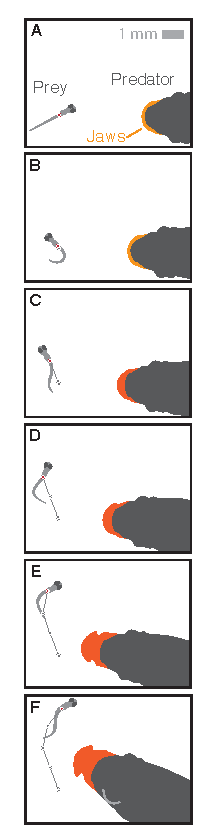
\includegraphics[width=1\textwidth]{Fig_01.pdf}
\centering	
\caption{\textbf{The Homicidal Chauffeur model, applied to prey strategy.} \textbf{(A)} Simulations predict the direction of a prey's fast start relative to initial position and velocity of a predator. \textbf{(B)} Numerical simulations were run at varying escape angle and predator approach speed to examine variation in the minimum distance. At $K>1$, the optimal angle. . .  }
\label{weihs_topo}
\end{centering}
\end{figure}

\pagebreak









% CLOSE DOCUMENT
\end{document}
